
\begin{figure}[t]
    \centering
    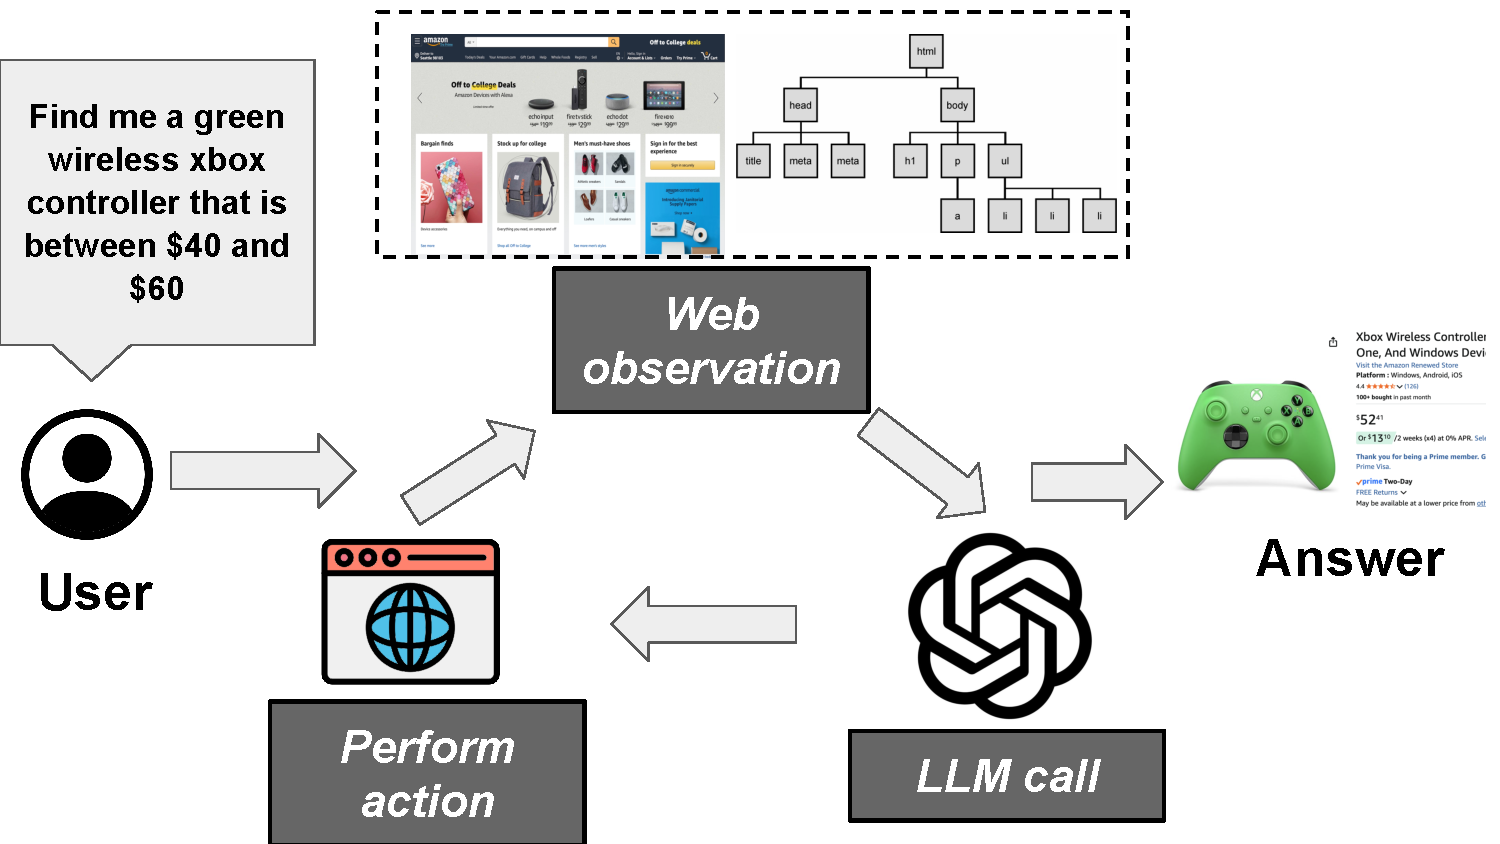
\includegraphics[width=0.8\columnwidth]{figures/5-4-2026/react-workflow.pdf}
    \tightcaption{Workflow of a representative ReAct-based web agent.
    The agent loops through render, observe, reason, and act steps
    until task completion.}
    \label{fig:react-workflow}
\end{figure}



\section{Background and Motivation}
\label{sec:background}

Web agents incur substantial overheads not intrinsic to their tasks. We examine where these overheads come from, identify the structural properties that make them avoidable, and characterize the challenges of automating their removal.





\begin{figure}[t]
    \centering
    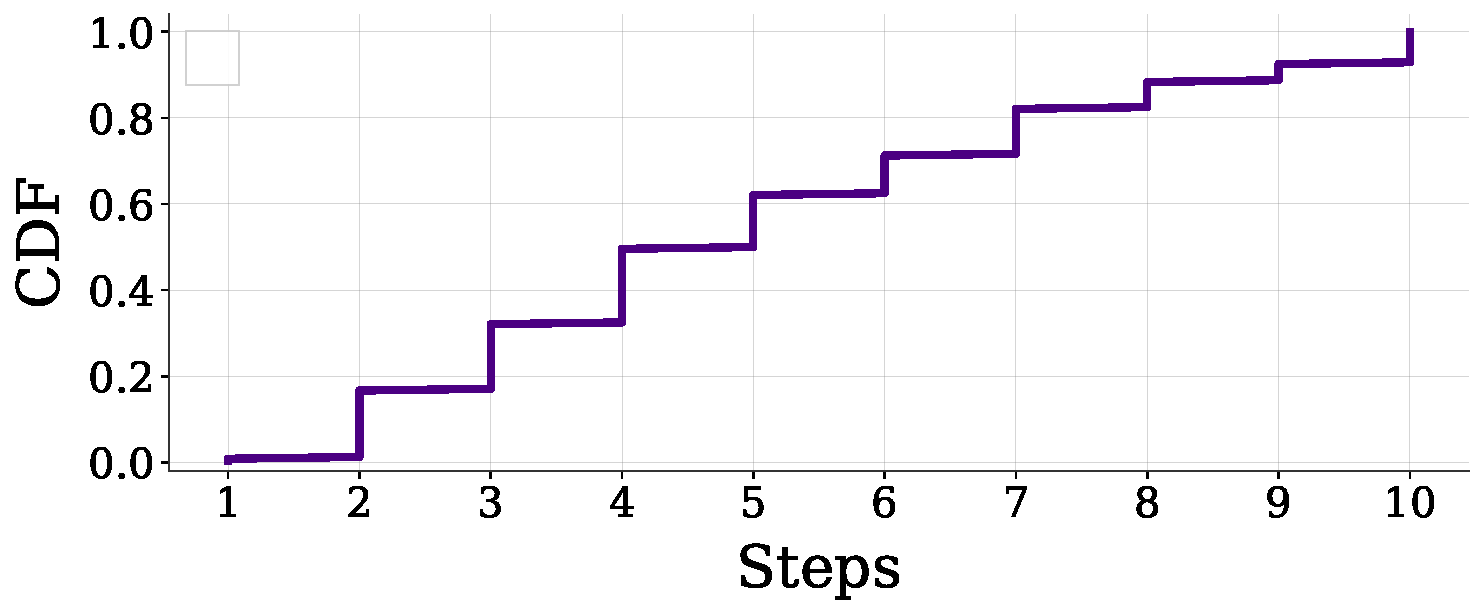
\includegraphics[width=0.8\columnwidth]{figures/steps_cdf.pdf}
    \tightcaption{Distribution of number of ReAct steps needed for agents to converge to an answer.}
    \label{fig:steps}
\end{figure}

\begin{figure}[t]
    \centering
    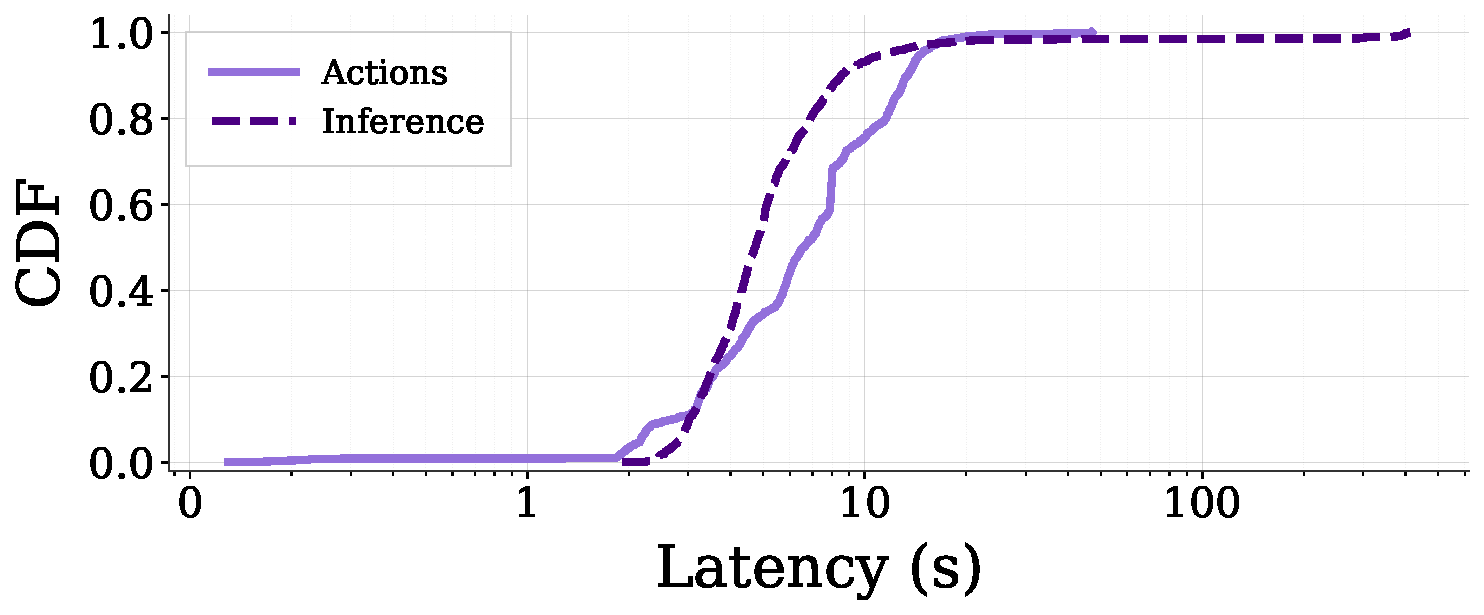
\includegraphics[width=0.8\columnwidth]{figures/latency_breakdown_cdf.pdf}
    \tightcaption{Per-step breakdown of latencies. Actions involve typing, clicking, googling, and scrolling while inference involves running the frontier model on the web input}
    \label{fig:latency-breakdown}
\end{figure}


\subsection{Overview of web agents}
\label{sec:bg}

Canonical web agents such as WebVoyager~\cite{webvoyager}, AgentOccam~\cite{agentoccam}, BrowserUse~\cite{browseruse}, and SeeAct~\cite{seeact} operate by coupling a frontier LLM with a headless browser through a ReAct execution loop~\cite{react} (Figure~\ref{fig:react-workflow}). At each step, the agent loads the current page in the browser, observes its rendered representation as either a serialized DOM tree or a screenshot, reasons about the next action to take, and executes that action against the page through standard browser primitives such as clicks, typed input, scrolling, and navigation. Every step requires a full LLM call that processes the current page representation alongside the running interaction history. The loop repeats until the agent decides the task is complete, deemed unachievable, or until a step budget is exhausted.

Web agents are designed for tasks that require navigating human-facing sites to retrieve targeted information. Example tasks include looking up product prices and availability across e-commerce catalogs, retrieving paper abstracts and citation counts from academic repositories, comparing course offerings across educational platforms, summarizing freshly-published news articles, and gathering reservation details from booking sites. They differ from tool-using agents that call structured APIs or MCP servers designed for programmatic access (e.g., coding agents acting on local files and developer tools~\cite{swt-bench, execution-agent}), and from stateless retrieval pipelines that synthesize answers from search-engine results without visiting the underlying pages~\cite{caesar}. The defining feature of a web agent is that it operates against the \emph{live web}, and must reason about page content and interaction patterns that vary across sites and across queries.


\subsection{Opportunities for specialization}
\label{sec:opp}

We start by profiling overheads across 151 representative tasks from the WebVoyager benchmark using three web agents -- BrowserUse, AgentOccam, WebVoyager -- and the experimental methodology outlined in \S\ref{sev:eval}.  Overall, we find that per-task latencies span 30-120 seconds, translating to per-task API costs of \$0.20-0.50 for model inference. Digging deeper, this overhead decomposes into two factors that each contribute substantially: the number of steps a trajectory takes, and the overhead of each step. As Figure~\ref{fig:steps} shows, the median task takes 4 steps with 80\% of tasks requiring at least 7 steps. Figure~\ref{fig:latency-breakdown} breaks down each step into browser actions and LLM inference delays, showing that both contribute meaningfully (median delays of 4.7 secs for LLM inference and 6.6 secs for browser action time, respectively). Since action decisions are conditioned on current page content and the trajectory thus far, per-step inference costs grow as history builds.



We argue that these overheads are not intrinsic to the underlying web agent tasks. Instead, they stem from applying heavy, general-purpose components -- frontier-model inference, full browser rendering, and the iterative ReAct loop, each designed for problems much broader than typical web agent tasks -- \emph{uniformly} across all steps regardless of need. We next describe three intrinsic properties of the web that make this uniformity unnecessary, and that together open the door to substantial specialization for acceleration.


\begin{figure}[t]
    \centering
    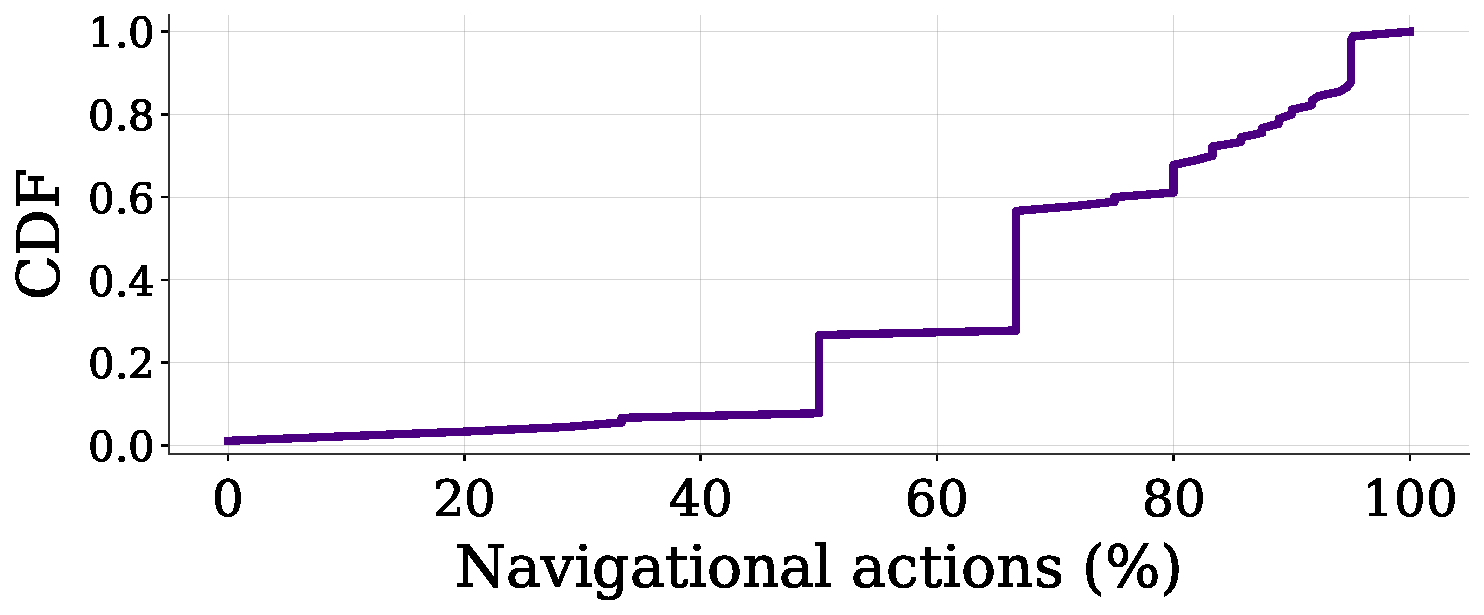
\includegraphics[width=0.8\columnwidth]{figures/navigational_actions_cdf.pdf}
    \tightcaption{Distribution of the percentage of steps per task that are navigational, i.e., moving the agent between pages rather than directly satisfying a task requirement by extracting an answer, comparing values, modifying page state.}
    \label{fig:navigational-actions}
\end{figure}

\begin{figure}[t]
    \centering
    
\includegraphics[width=0.8\columnwidth]{figures/excessive-data-2.pdf}
    \tightcaption{Web state input at one step of a task. Red circle marks the search bar, the only
element load-bearing for the next action (typing the query). The
rest of the input (product recommendations,
images, sidebar links, etc.) is not needed.}
    \label{fig:excessive-data}
\end{figure}


\para{Most steps are navigational.}
Most web agent tasks involve read-only information retrieval (a product price, a paper's citation count, a course's prerequisites), with the answer typically concentrated on one or a few destination pages. Reaching those pages involves searching, filtering, paginating, clicking through results, and so on. However, these steps are primarily navigational -- steps used to move between pages rather than to directly satisfy a task requirement -- rather than load-bearing reasoning. Figure~\ref{fig:navigational-actions} illustrates this, showing that 66.7\% of steps are purely navigational for the median task in our benchmarks. Further, on a given site, this navigation often follows query-invariant patterns: every Amazon shopping task involves search-then-product-page navigation, every arXiv lookup resolves an identifier to an abstract page, every GitHub task locates a repository by owner and name. An agent that knows the pattern can thus reach the destination in a single direct fetch rather than rediscovering it via a multi-step ReAct loop, with only the query-specific identifiers substituted in.

%Most web agent tasks involve read-only information retrieval (a product price, a paper's citation count, a course's prerequisites), with the answer typically concentrated on a single destination page. Reaching that page involves searching, filtering, paginating, clicking through results, and so on. However, these steps serve primarily as navigational scaffolding for interaction intuitiveness, rather than load-bearing reasoning. Further, on a given site, task-level navigation often follows query-invariant patterns: every Amazon shopping task involves search-then-product-page navigation, every arXiv lookup resolves an identifier to an abstract page, every GitHub task locates a repository by owner and name. Figure~\ref{fig:navigational-actions} illustrates this, showing tha\fillin{X\%} of steps for the median task in our benchmarks involves actions whose sole purposes is to traverse the site without extracting information or modifying page state. An agent that knows the pattern can therefore reach the destination in a single direct fetch rather than rediscovering it through a multi-step ReAct loop, with only the query-specific identifiers substituted in. 


% \begin{figure}[t]
%     \centering
%     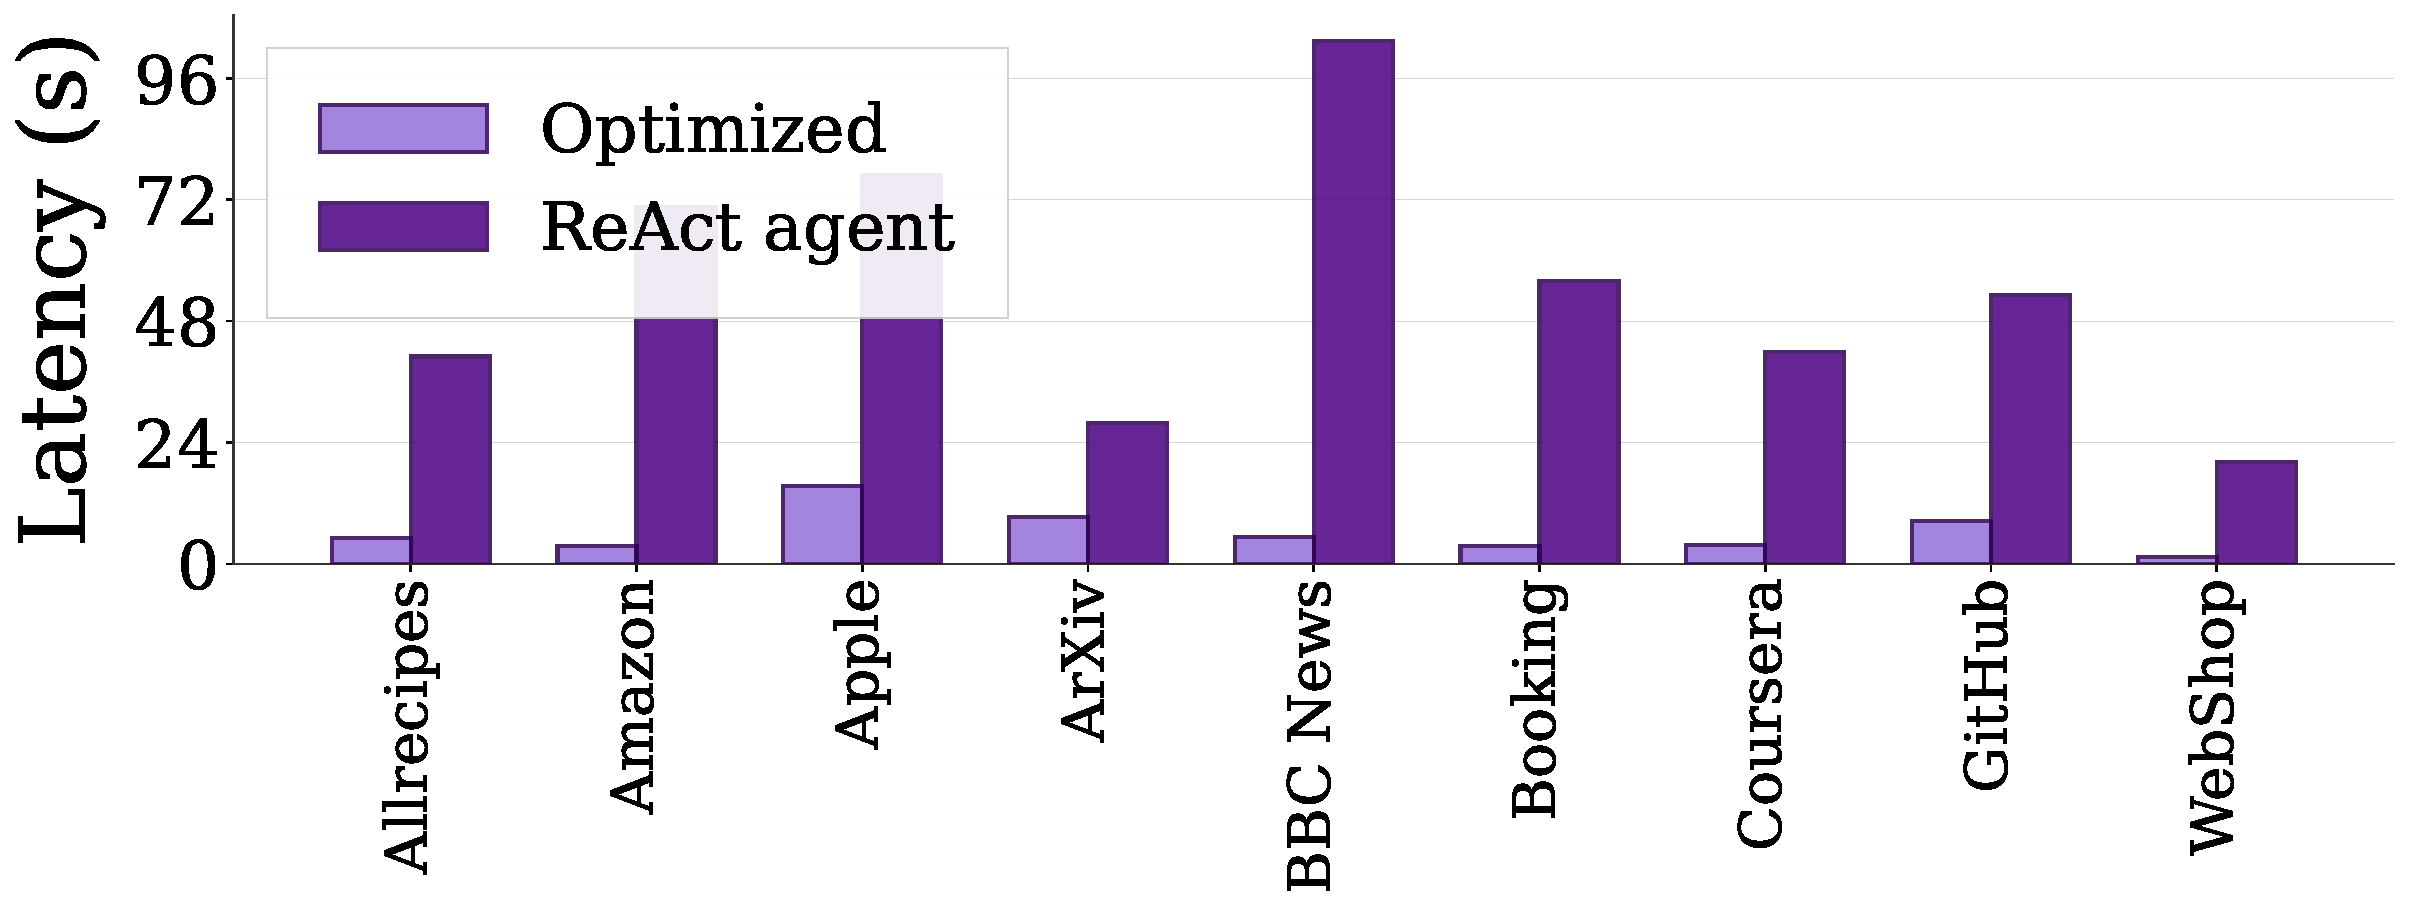
\includegraphics[width=0.99\columnwidth]{figures/hand_optimized_motivation.pdf}
%     \tightcaption{Latency of handcrafted optimized programs versus an
% off-the-shelf ReAct agent on nine representative tasks across
% diverse sites. Handcrafted programs run roughly an order of
% magnitude faster by skipping steps and using only the resources
% each task needs.}
%     \label{fig:hand-optimized}
% \end{figure}


\begin{figure}[t]
    \centering
    \begin{minipage}{0.48\columnwidth}
        \centering
        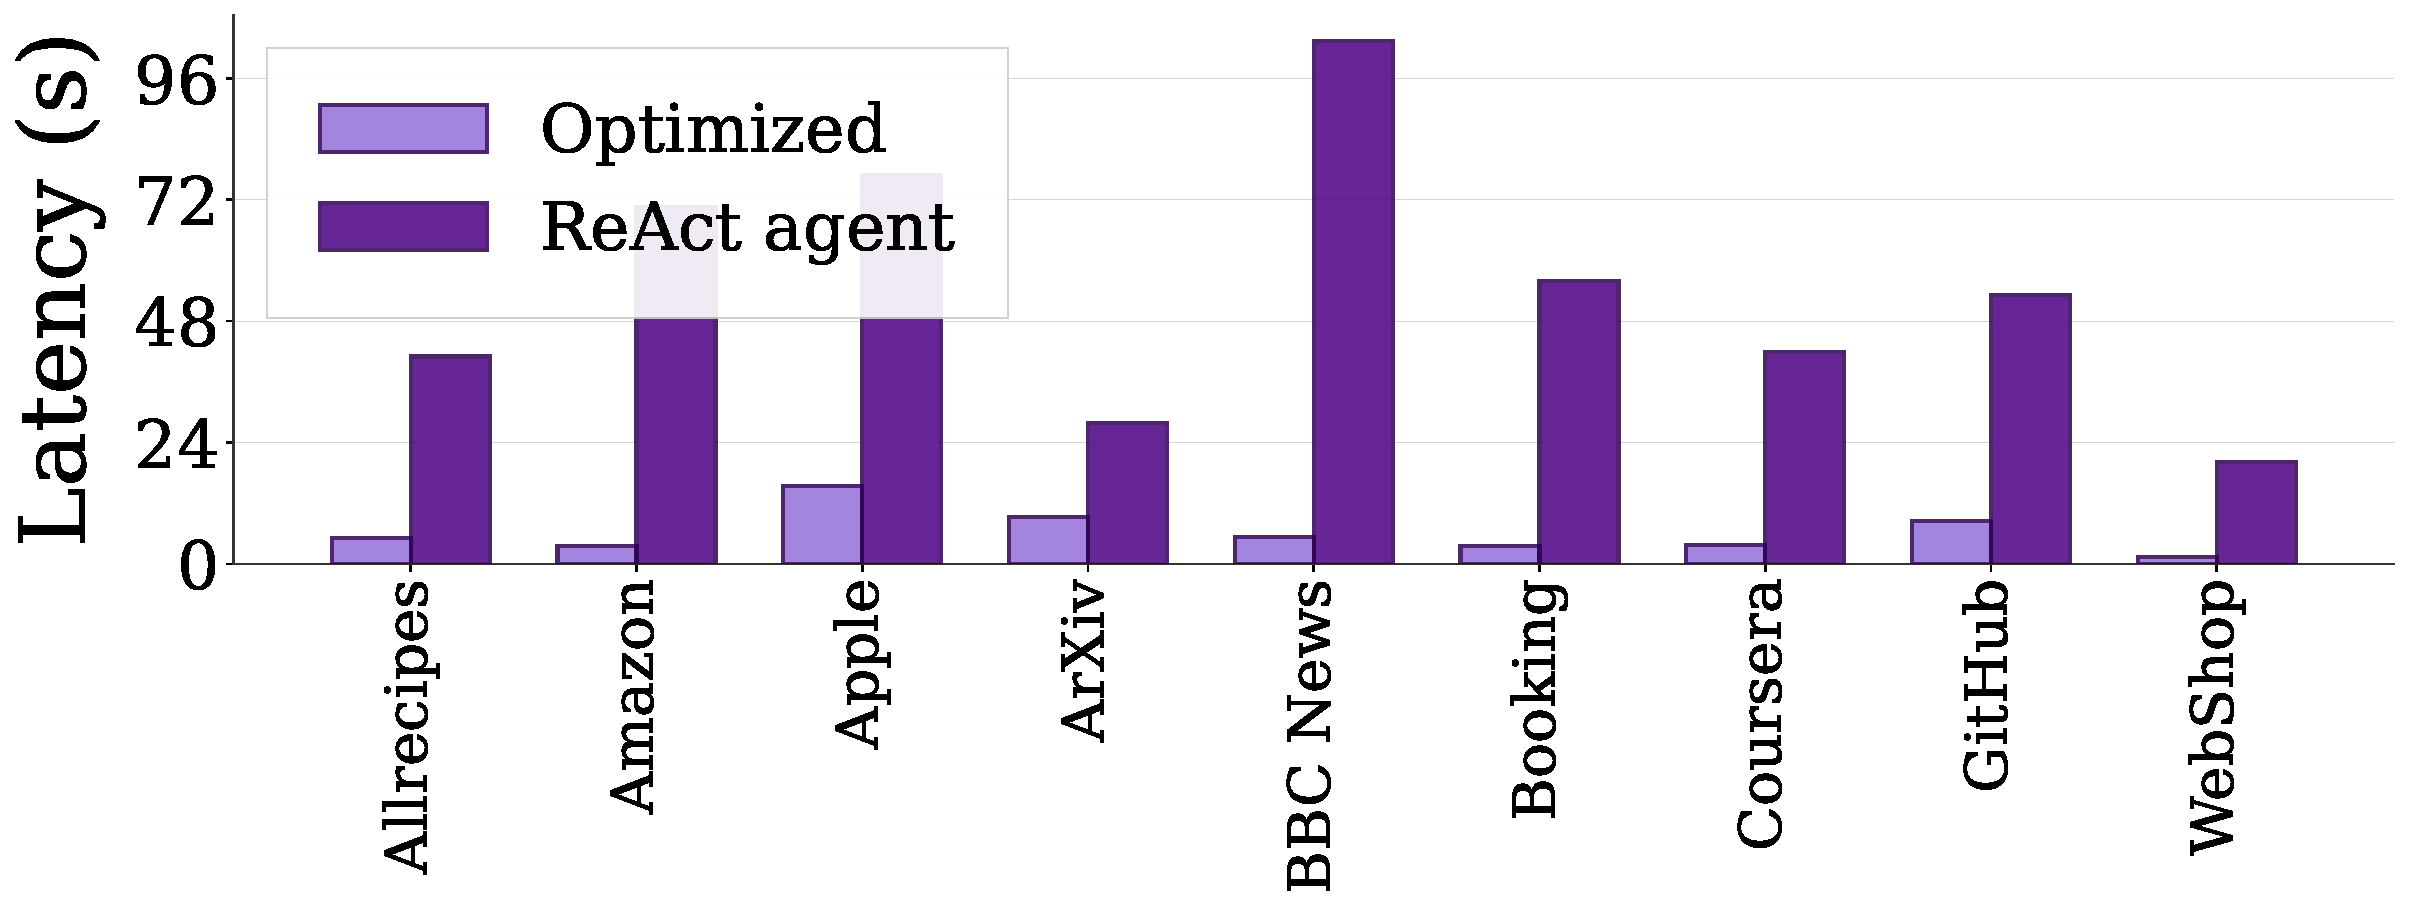
\includegraphics[width=\linewidth]{figures/hand_optimized_motivation.pdf}
        \tightcaption{Latencies of handcrafted optimized programs.}
        \label{fig:hand-optimized-latency}
    \end{minipage}
    \hfill
    \begin{minipage}{0.48\columnwidth}
        \centering
        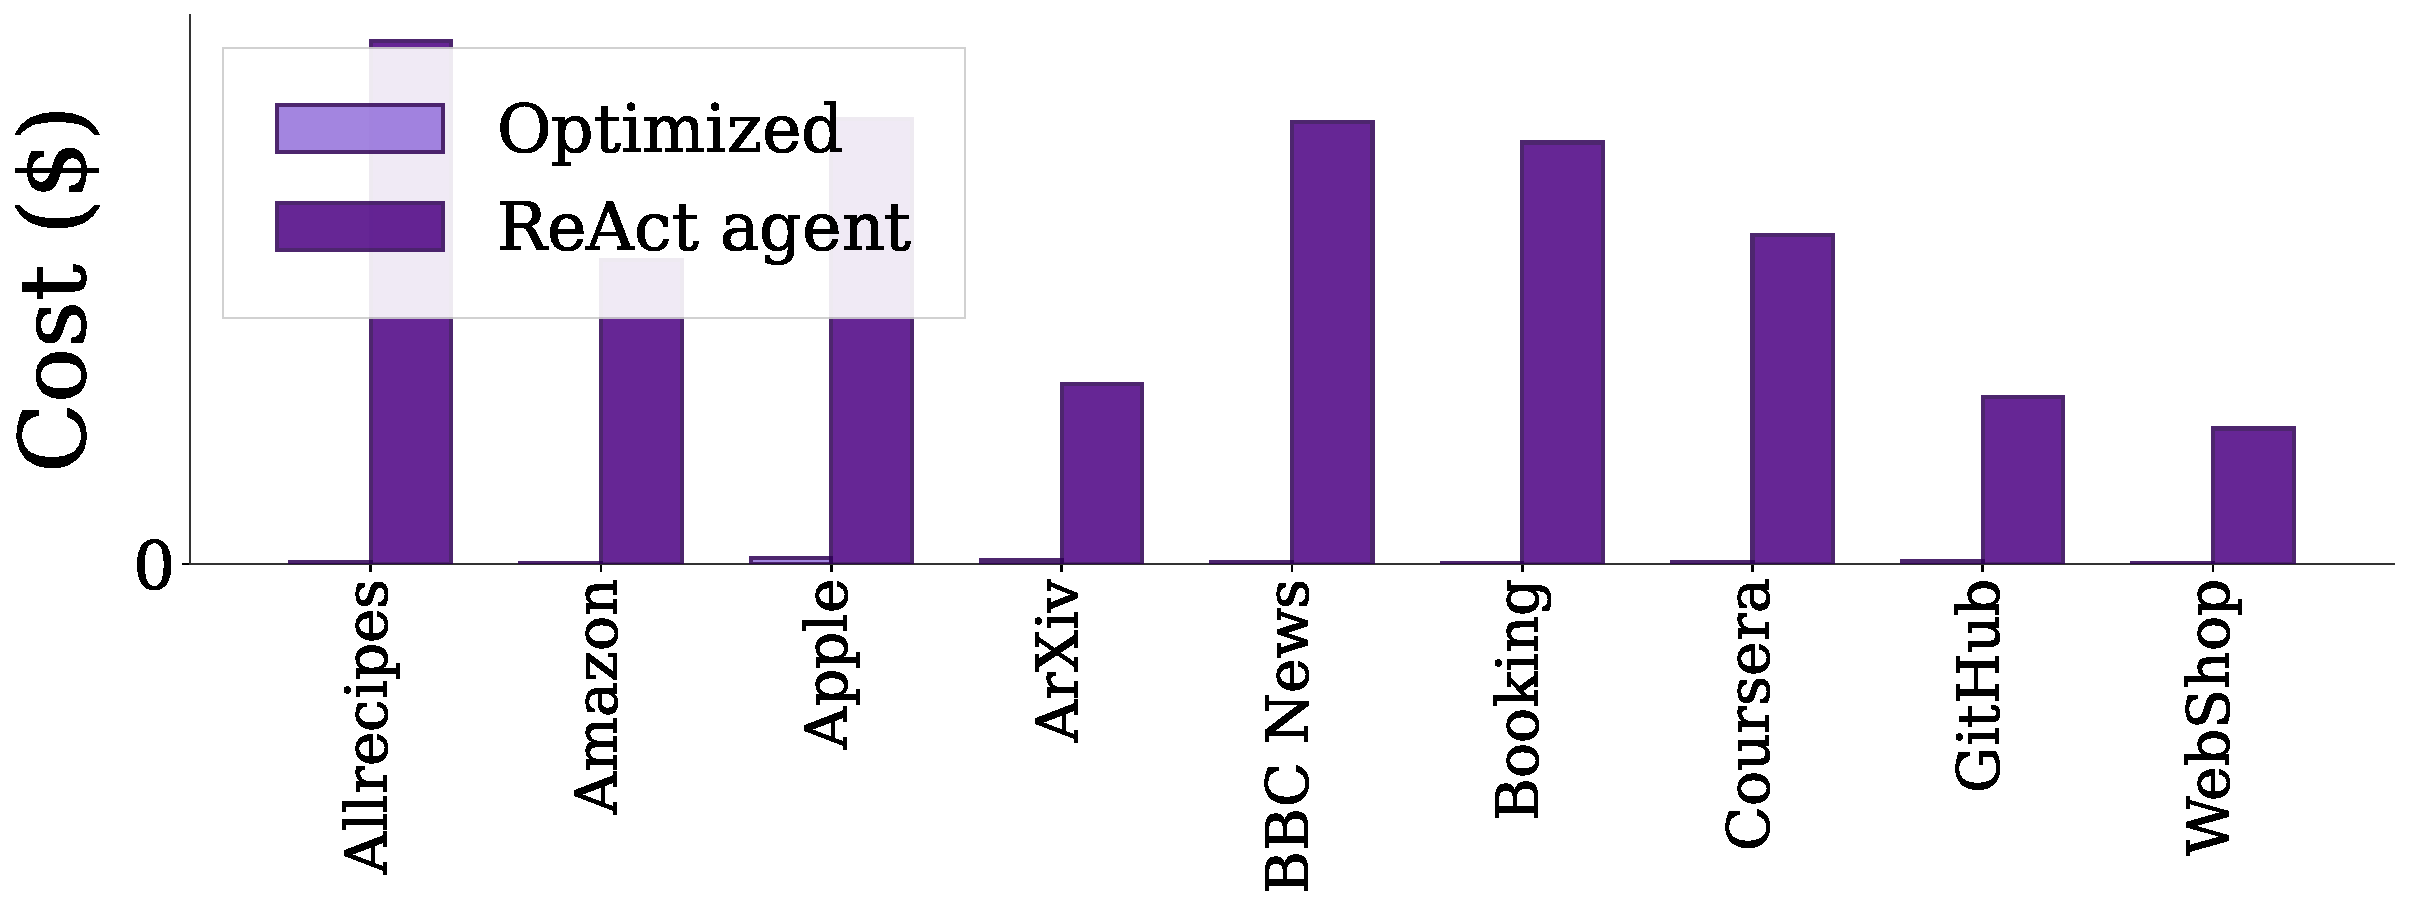
\includegraphics[width=\linewidth]{figures/hand_optimized_costs_motivation.pdf}
        \tightcaption{Costs of handcrafted optimized programs.}
        \label{fig:hand-optimized-cost}
    \end{minipage}
\end{figure}




\begin{figure}[t]
    \centering
    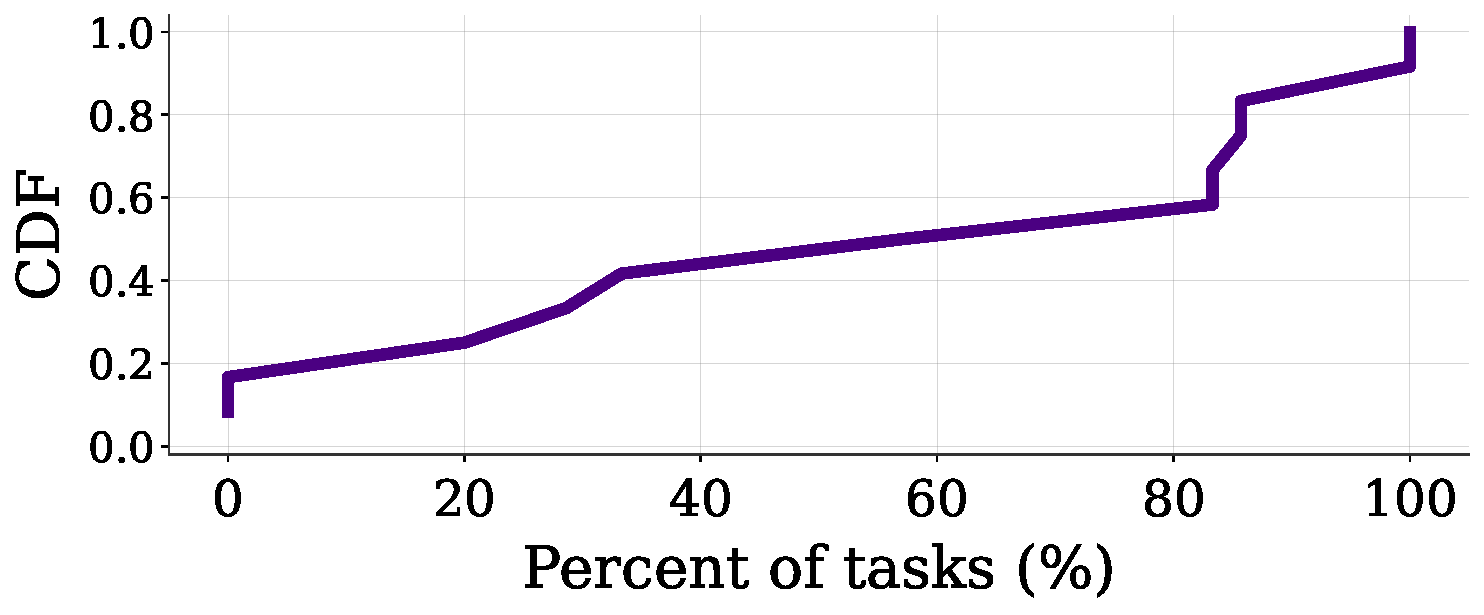
\includegraphics[width=0.8\columnwidth]{figures/http_coverage_cdf.pdf}
    \tightcaption{Fraction of tasks per site solvable via HTTP-only execution. Many sites support a large percentage of tasks through direct retrieval without browser interaction.}
    \label{fig:http-coverage}
\end{figure}

\para{Many pages do not need a browser.}
For many sites, the content embedding a task's answer is rendered on the server and arrives complete in the HTTP response body (e.g., Amazon product pages, arXiv abstracts, GitHub repository views). In these cases, a plain HTTP fetch returns what the browser would have displayed, without the high overheads of scripting and rendering. Figure~\ref{fig:http-coverage} confirms that this is common: for 55.8\% of tasks in our benchmark, the content necessary to resolve the query is fully accessible via HTTP fetch alone, without invoking the browser. Browser execution remains necessary only when client-side JavaScript produces load-bearing content (e.g., interactive maps, dynamically-revealed product variants), and even then, these overheads are warranted only for the specific steps that depend on the dynamically-generated content. Skipping even a subset of browser executions can eliminate substantial overhead.

\begin{figure}[t]
    \centering
    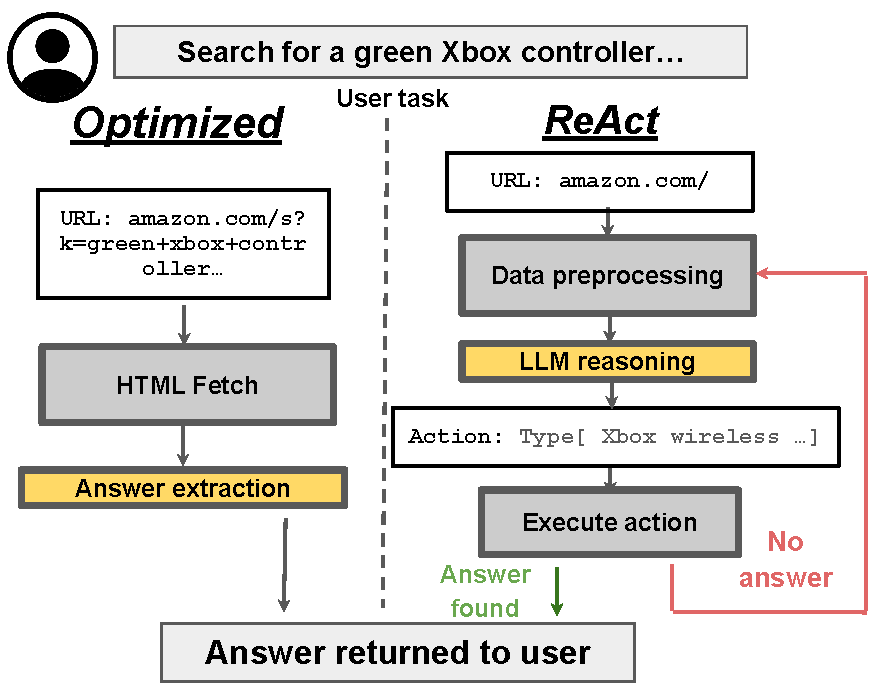
\includegraphics[width=0.8\columnwidth]{figures/optimized-web-program.pdf}
    \tightcaption{Comparison of a hand-optimized program (left) and the
corresponding off-the-shelf ReAct trajectory (right) for an
Amazon retrieval task. }
\vspace{4pt}
    \label{fig:optimized-web-program}
\end{figure}

%\para{Many pages do not need a browser.}
%For many sites, the content embedding a task's answer is rendered on the server and arrives complete in the HTTP response body (e.g., Amazon product pages, arXiv abstracts, GitHub repository views). In these cases, a plain HTTP fetch returns what the browser would have displayed, without the high overheads of scripting and rendering. Browser execution remains necessary only when client-side JavaScript produces load-bearing content (e.g., interactive maps, dynamically-revealed product variants), and even then, these overheads are warranted only for the specific steps that depend on the dynamically-generated content. Skipping even a subset of browser executions can eliminate substantial overhead in the agent's stack.


%Browsers are engineered to render arbitrary client-side behavior, much of which rarely contributes to the textual content an extraction model needs, e.g., GUI layout, click handling, hover effects, animation, JavaScript execution. Some client-side execution does produce load-bearing content (e.g., interactive maps, dynamically-revealed product variants), but for many read-only sites the answer-bearing content is server-rendered and arrives complete in the HTTP response body. A plain HTTP fetch therefore returns what the browser would have displayed on those sites. Even on sites where some pages require client-side rendering, direct-URL fetches still skip much of the trajectory, with browser execution invoked only for the steps that genuinely require it. The browser is the heaviest component in the agent's stack — both in per-step latency and in operational overhead — and many steps need none of what it provides.


%Browsers are engineered to render arbitrary client-side behavior that primarily exists to serve human interaction, e.g., GUI layout, click handling, hover effects, animation, JavaScript execution. For most read-only sites, the answer-bearing content is server-rendered and arrives complete in the HTTP response body, so a plain HTTP fetch returns what the browser would have displayed. Browser execution remains necessary for the minority of pages whose load-bearing content is produced by client-side JavaScript (e.g., interactive maps, dynamically-revealed product variants), but even on these sites, the steps that depend on browser rendering are a small fraction of the trajectory. The browser is the heaviest component in the agent's stack — both in per-step latency and in operational overhead — and most steps need none of what it provides.

%  \begin{figure}[t]
%      \centering
%      \includegraphics[width=0.9\columnwidth]{figures/denoised_motivation_bar.pdf} 
%           \tightcaption{Effect of page noise on extraction accuracy. Qwen2.5-14B matches GPT-4o on small, denoised page content embedding only the necessary information, but degrades sharply on full pages while GPT-4o remains comparatively robust.}
% %     % \tightcaption{\fillin{Accuracy with small and frontier models as additional page content not relevant to the step goal is considered during inference.}}
%      \label{fig:accuracy-vs-noise}
%  \end{figure}

 \begin{table}[t]
    \centering
    \small
    \begin{tabular}{lcc}
        \toprule
        \textbf{Model} & \textbf{Denoised environment} & \textbf{Full environment} \\
        \midrule
        Qwen2.5-14B & 42.7\%  & 26.1\%  \\
        GPT-4o &  45.7\% & 45.0\% \\
        \bottomrule
    \end{tabular}
    \vspace{8pt}
    \tightcaption{Effect of page noise on extraction accuracy. Qwen2.5-14B matches GPT-4o on small, denoised page content embedding only the necessary information, but degrades sharply on full pages while GPT-4o remains comparatively robust.}
        \label{t:accuracy-vs-noise}
\end{table}

\para{Most steps do not need a frontier model.}
A typical web page presents hundreds of potential actions in the form of interactive elements alongside ads, recommendation widgets, navigation chrome, and related-content sidebars (Figure~\ref{fig:nav-elements-challenge1}). However, the content directly relevant to a given step (e.g., a price, an abstract, a commit count) often occupies only a small fraction of the page's DOM content; Figure~\ref{fig:excessive-data} shows an illustrative example. Powerful frontier models are necessary to reason over this combination of useful content and noise, but the underlying extraction -- i.e., locating and returning the page content relevant to the step -- is not inherently hard. The relevant region is not only small but predictably located: a product's price routinely appears in the same place across product pages, an ArXiv abstract appears in the same place across paper pages, etc. Once that region is isolated, extraction reduces to a structured task within a smaller model's competence. 
Table~\ref{t:accuracy-vs-noise} confirms this empirically: when presented only with the region of a page embedding the answer (i.e., `denoised'), non-frontier models nearly match frontier-model accuracy; on full pages, however, non-frontier accuracy plummets while frontier models remain capable. 

%Powerful reasoning models have the ability to reason over the abundance of content and hundreds of action choices in a typical page (Figure~\ref{fig:accessibility-tree}) to robustly decide what to do next. However, despite the array of information that pages embed (e.g., ads, recomendation widgets, sidebars), the content directly related to the step at hand (e.g., a price, an abstract, a commit count) typically occupies a very small fraction of the page's DOM. (Figure~\ref{fig:excessive-data} provides an example). This observation has direct implications on inference costs: pages are organized so that any given query's answer often lives in a small, predictable region of the page, and once that region is isolated, the extraction itself is a structured task within a smaller model's competence. Figure~\ref{fig:accuracy-vs-noise} confirms this empirically, showing that small models rival accuracies of their frontier counterparts when presented only the necessary page content for a step, but unlike frontier models, their accuracy quickly degrades as the surrounding (noisy) page content they are presented with grows. 

%are necessary when an agent must reason over a noisy, unstructured page to decide what to do next: a typical page (Figure~\ref{fig:accessibility-tree}) presents hundreds of clickable elements alongside ads, recommendation widgets, navigation chrome, and related-content sidebars, with the step-related content (a price, an abstract, a commit count) occupying a small fraction of the DOM. The difficulty is one of noise tolerance, not of the underlying extraction: pages are organized so that any given query's answer lives in a small, predictable region of the page, and once that region is isolated, the extraction itself is a structured task within a smaller model's competence. Figure~\ref{fig:accuracy-vs-noise} confirms this empirically. When given only the answer-bearing region of a page, non-frontier models match frontier-model accuracy; as surrounding noise is added, non-frontier accuracy degrades while frontier accuracy remains roughly flat. The full-page noise is what forces frontier models in the first place. An agent that filters page content against an expected answer structure can therefore replace frontier inference with non-frontier inference on the resulting focused subset.

\para{Opportunity.}
To quantify the savings these three properties enable, we hand-engineer specialized programs for nine representative tasks in the WebVoyager benchmark. Each program implements the same recipe illustrated in Figure~\ref{fig:optimized-web-program}: a per-site URL template constructs the target page URL, an HTTP request fetches the page, the HTML is filtered to the answer-bearing region encoded by the site's expected answer structure, and a non-frontier model (i.e., Qwen2.5-14B-Instruct rather than GPT-4o/GPT-5) extracts the answer. As Figures~\ref{fig:hand-optimized-latency} and \ref{fig:hand-optimized-cost} shows, these fast-path programs run 66.7-94.9\% faster 17.7-100.7$\times$ lower costs) than the off-the-shelf ReAct agent, while preserving accuracy.

\begin{figure}[t]
    \centering
    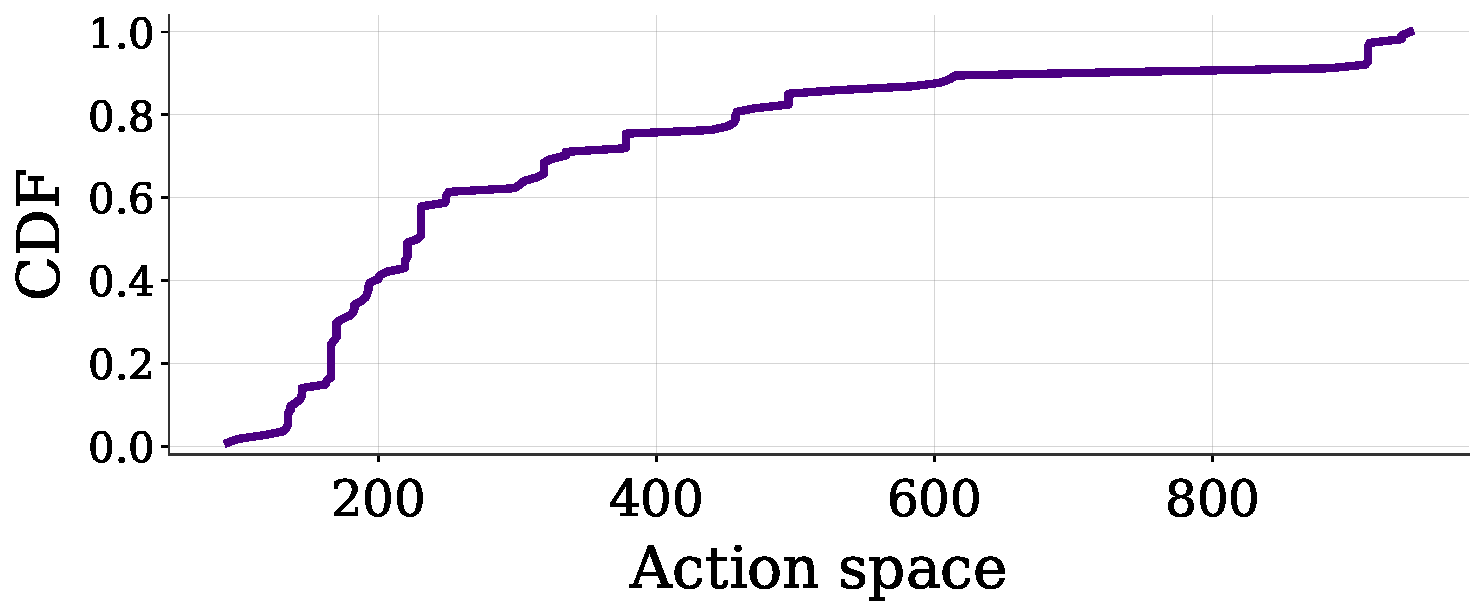
\includegraphics[width=0.8\columnwidth]{figures/action_space_count_cdf_challenge_1.pdf}
    \tightcaption{CDF of navigational elements (links, buttons, form
inputs) per page across ReAct trajectories. The median page
presents 212+ navigational elements, each leading to a different
page. }
    \label{fig:nav-elements-challenge1}
\end{figure}


\begin{figure}[t]
    \centering
    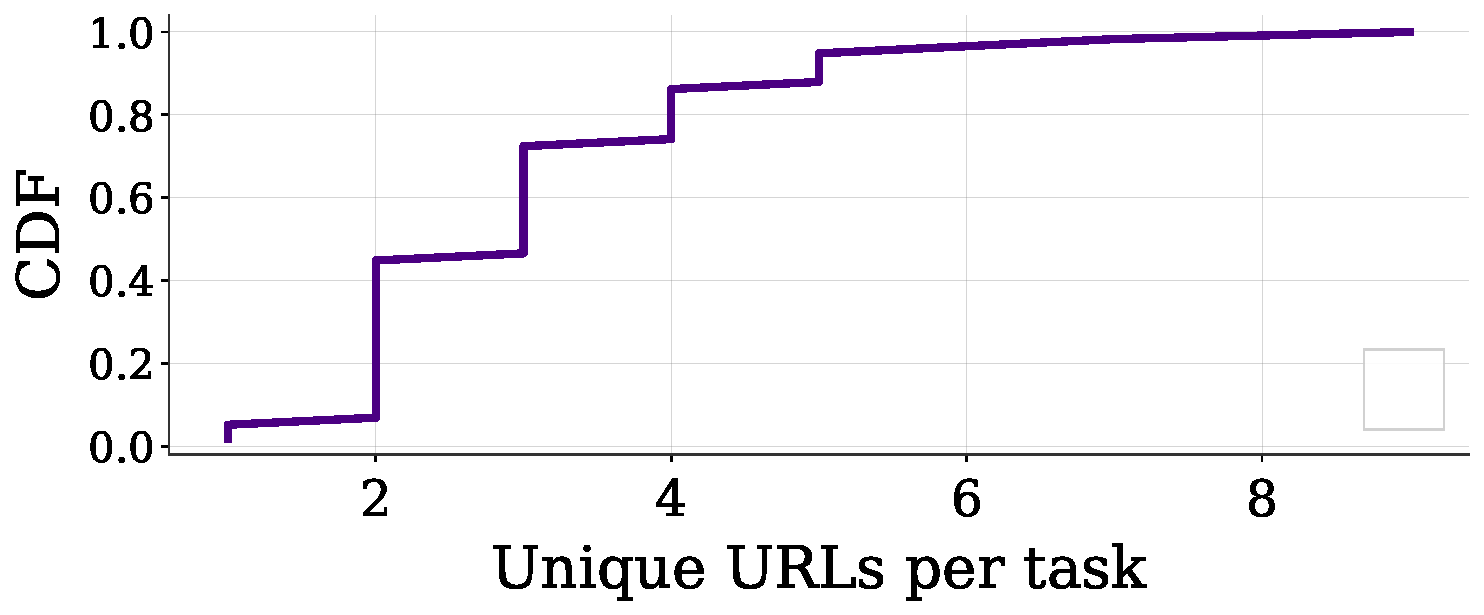
\includegraphics[width=0.8\columnwidth]{figures/unique_per_task_url_cdf_challenge1.pdf}
    \tightcaption{Number of unique URLs visited by each task. Tasks tend to take very different trajectories. Note that multiple steps often occur within each URL (e.g., scrolling) }
    \label{fig:unique-per-task-url-cdf-challenge1}
\end{figure}


\begin{figure}[t]
    \centering
    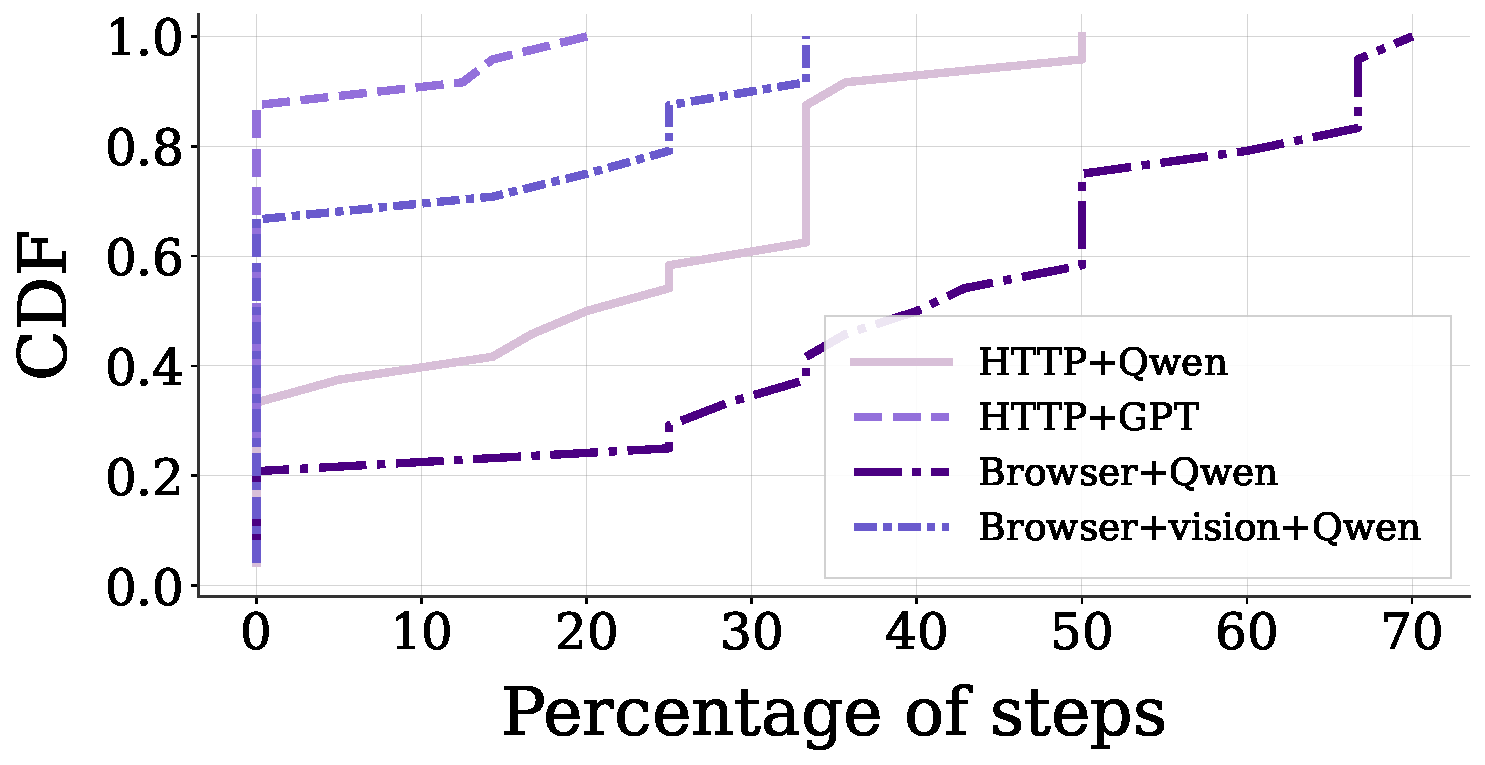
\includegraphics[width=0.8\columnwidth]{figures/minimum_tier_required_challenge_2.pdf}
    \tightcaption{CDF over tasks of the percentage of steps requiring each compute tier as the weakest tier sufficient to match the full ReAct agent. Tiers combine page-fetch (HTTP, browser, or browser w/ screenshot) with a model (Qwen2.5-14B or GPT-4o).}
    \label{fig:minimum-tier-required-challenge2}
\end{figure}

\subsection{Challenges}
\label{sec:chal}

Automatically realizing the promise of specialization above requires overcoming two key challenges, which we describe in turn. The cost of getting either wrong is severe: naively substituting cheap components (a non-frontier model and HTTP fetch) into the off-the-shelf ReAct loop, without the URL templates and answer schemas that hand-engineered programs encode, drops average task success by 60\% since errors compound across the trajectory and a single wrong step can invalidate everything downstream.

%The cost of getting either wrong is severe: naively applying the recipe of fast optimizations in Figure~\ref{fig:optimized-web-program} to the off-the-shelf ReAct loop drops task success to 0\%, since errors compound across the trajectory and a single wrong step can invalidate everything downstream.


\para{C1: Determining \emph{what} can be specialized.}
Before execution begins, the agent must determine which parts of an incoming task support specialization, i.e., which trajectories can be replaced by direct URL fetches, which pages can be served without a browser, and which extraction steps can use a non-frontier model. This determination is hard for two reinforcing reasons. First, the signal available at query time is thin. Task text describes user intent (``find the cheapest blue headphones'') rather than the trajectory pattern that resolves it, and even on a single site, different tasks visit different pages through different navigation sequences. Second, recognition itself has a cost ceiling: if identifying reuse opportunities requires running a frontier model over the full site or comparing against a large trajectory database, the cost of recognition negates the savings that the specialization would yield. The challenge is thus how to encode reusable site structure ahead of time and match incoming tasks against it efficiently at runtime.

%\emph{robustly} surface reusable site structure ahead of time and recognize when an incoming task matches it cheaply enough that the savings remain meaningful.


\para{C2: Determining \emph{how} to specialize across steps.}
Even when specialization applies, the minimum-cost \emph{tier} -- a combination of retrieval, rendering, and extraction model -- sufficient to match the default agent varies per step within a single trajectory. Figure~\ref{fig:minimum-tier-required-challenge2} highlights this by showing the distribution of minimum-tier support needed across task steps. As shown, some steps are resolved by the cheapest tier (HTTP fetch with a non-frontier model), others require browser rendering to access client-side content, others require a frontier model for extraction the small model cannot perform, and some require both. Importantly, the variation is \emph{per step}, not just per task; even tasks amenable to specialization mix step types within their trajectories. Choosing the wrong tier at any step drops accuracy substantially. For instance, a small model handed a raw DOM with a complex extraction task might return the wrong field, while an HTTP fetch of a JavaScript-dependent page will return a content stub without the necessary information. The challenge is to determine the minimum sufficient tier per step without paying the cost of running the default agent to find out.


